% !TEX root = ../main.tex
This section will analyze and describe the problems, which was introduced in the introduction section, into greater detail. 
~\\

The validation of reports is a problem, as we assume that municipality workers have to spend time reading through reports, and validate them either based on submitted images, or travel to the location of the report to personally validate it. This process seems very time consuming and like a waste of municipality resources.

\begin{figure}[hbt]
\centering
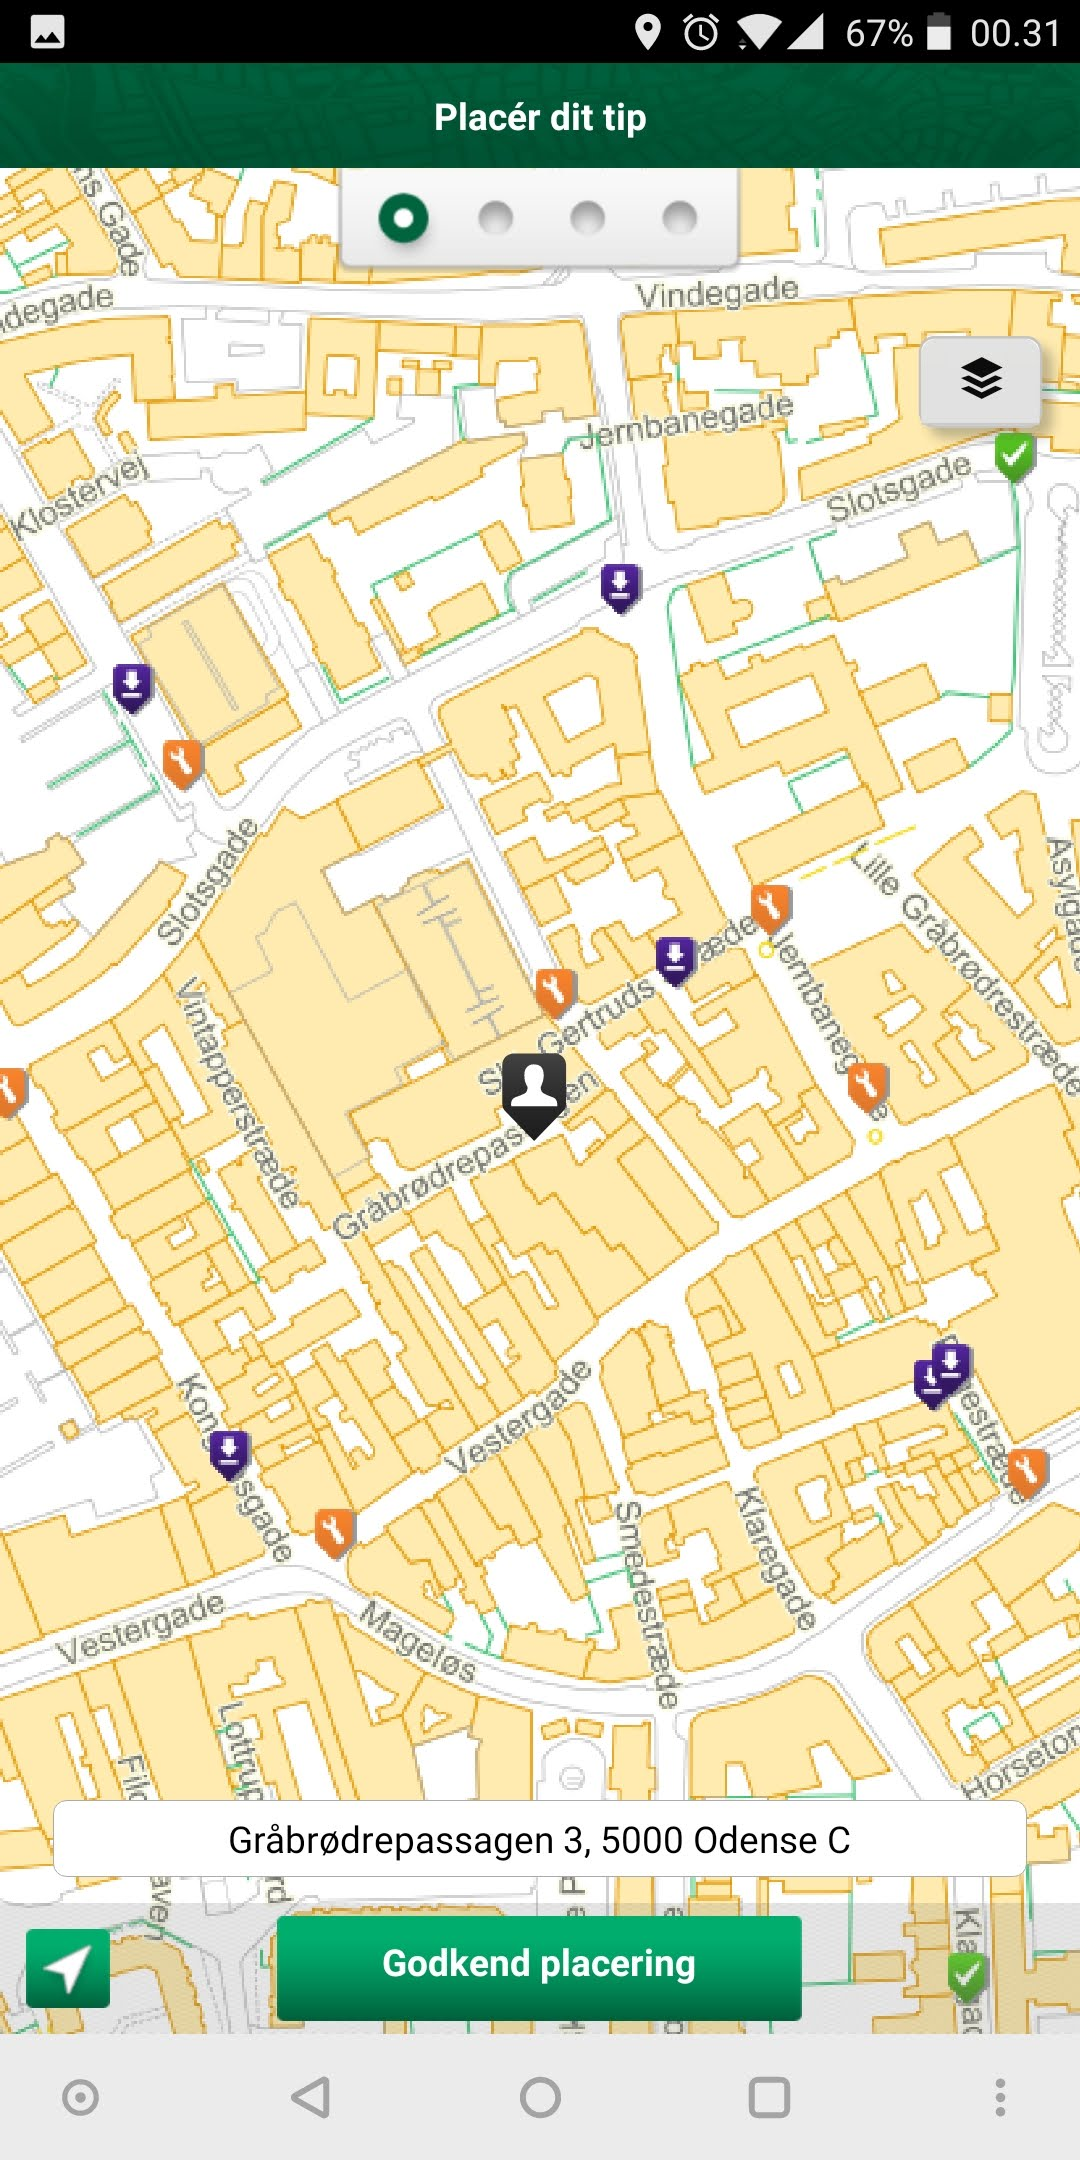
\includegraphics[width=5cm]{images/giv_et_tip_current_scr}
\caption{Image of the map screen in the current application.} \label{fig:current_app}
\end{figure}

In the current application, as \autoref{fig:current_app} shows, it is possible to see where other reports has been created, but there seems to be no way to get any information about these reports, other than the icons showing the report status.

The municipality also have a website which shows an overview of the current reports, but again, it does not offer any other functionality, for users to interact with the already reported issues. In order to contribute data to an already reported issue a user has to create a duplicate report with some more (accurate) information. This will eventually lead to more reports that the municipality workers have to validate.
~\\

The prioritization of reports is a problem, as we assume that the municipality workers have to dig through multiple reports and prioritize them. This process can cause a potentially dangerous issue, or an issue which affects more citizens, to become buried between the many other reports. 
~\\

The platform lacks an incentive for the users to use the platform, other than it being an easier way to report issues with. If there is no incentive to use the application, the amount of active users on the platform will decrease over time, which will result in a decrease in the amount of reports the municipality will receive.

\vspace{3em}

\hrule

This section has described the three problems that the project will try to solve. The solution for these problems will be elaborated upon in the next section.
